\chapter{背景與挑戰}
\label{chapter:background}


行動網路主要分成接入端網路 (AN, access network) 與核心網路 (CN, core network),其中接入端最常見的形式便是以基地臺 (base station) 為主的無線網路接入 (RAN, radio access network),主要負責聯接使用者設備 (UE, user equipment) 與核心網路、訊號解碼、波束成型、協助核網進行移動管理等等功能,包含 3G 時期的 nodeB、4G 時的 eNodeB、與 5G 時的 gNodeB。核心網路則是負責處理除接入端外剩下所有事務,包含認證、行動管理、服務品質管理、封包轉送、用量計費、連線與路由規劃、使用者資料紀錄等等功能,包含 2/3G 時的 GPRS 核心網路、4G 的 EPC、與 5G 的 5GC。而核心網路之外會接入資料網路 (DN, data network),包含但不限於我們常見的網際網路 (the Internet) 或電信商可能會提供的 MEC 網路。完整架構可參考圖~\ref{fig:5g_core_arch},此為 3GPP 於 23.501~\cite{3gpp.23.501}標準定義之 5G 行動網路架構圖。

本章我們會著墨於 5G 核心網路的介紹,包含用戶層與控制層的介紹,以及常見流程,然後介紹並比較幾個知名的 5G 核心網路專案,最後會描述目前 5G 核心網路所遇到的挑戰。

\begin{figure}[htbp]
    \centering
    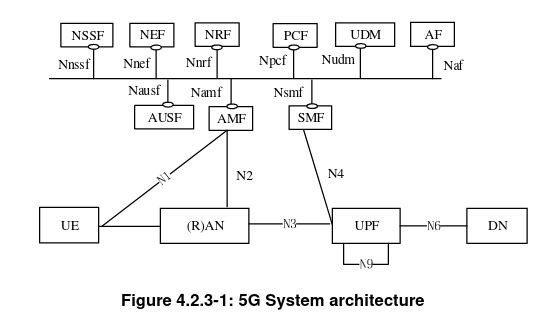
\includegraphics[height=!,width=1\linewidth,keepaspectratio=true]
                    {figures/23_501_4-2-3-1_sys_arch_sbi}
                    % [] 放的是顯示在 list of figure 的文字
                    % {} 放的是顯示在圖下方的文字
                    \caption[5G 核網架構]{{\footnotesize 5G 核網架構 (取自 TS 23.501 Figure 4.2.3-1~\cite{3gpp.23.501})}}
                    \label{fig:5g_core_arch}
\end{figure}
\pnote{圖片自畫}

\section{5G 核心網路架構}
\label{sec:5g_core}

% 介紹功能 CUPS、SBI、NF、NFV
要瞭解 5G 核心網路首先要對 4G 核心網路有一些概念,在 4G 時代,核心網路主要有幾個重要的部件 (component),Mobility Management Entity (MME)、Serving Gateway (S-GW)、PDN Gateway (P-GW)、Home Subscriber Server (HSS)、與 Policy and Charging Rules Function (PCRF) (見圖~\ref{fig:4g_core_arch},這裡不討論其他額外功能),MME 負責連線與移動的管理,S-GW 負責與 RAN 對接,將 LTE 的承載 (bearer) 轉換成 Internet 的形式,P-GW 負責與網際網路間接,HSS 會紀載使用者資料與幫助認證,PCRF 則是作規則與計價的管理。而隨著 4G 行動網路的發展,3GPP 會議與電信商越加越多新的功能後,發現此架構不再適用於新功能的發展,而決定對核心網路有架構性的改變,而發展出了 5G 核心網路。5G 核心網路在架構上有幾個突破性的改變,包含:
\begin{itemize}
    \item \textbf{網路功能虛擬化 (NFV, Network Function Virtualization):} 核心網路爲應印雲端 (cloud) 與微服務 (microservice) 的架構,逐漸往網路功能虛擬化方向發展,及所以功能部件皆以軟體形式呈現以方便於在標準化硬體 (commodity hardware) 上部屬,並且核心網路亦將 4G 的五大部件依據功能性,拆分為更小的單位,並以 Network Function 稱之 (以下簡稱 NF)。
    \item \textbf{用戶端與控制端分離 (CUPS, Control and User Plane Separation):} 4G 時如 S/P-GW 同時具備用戶端功能與控制端功能,但在逐漸發展後,3GPP 認為應該將用戶端與用戶端分離,於是研議出 4.5G 時的 CUPS,將 S/P-GW 的用戶端功能拉出並以 PFCP (Packet Forwarding Control Protocol) 協定控制,而 5G 時更是把 S/P-GW 的使用者功能合併並獨立拉出成一個 NF。
    \item \textbf{服務導向架構 (SBA, Service Base Architecture):} 有鑑於 5G 將核網區分為更多小單位的 NF,如此多種不同整類的 NF 若需互相溝通,將需要開發出多種不同的界面與協定而導致開發與擴展困難,因此 3GPP 於 5G 時採用 SBA 架構,其界面統稱為 SBI (Service Base Interface),透過制定統一的通訊格式,減少需要對每個界面開發出新協定的繁瑣,並且若需要新增界面或 NF,僅需重新使用相同格式便可輕鬆開發出新的界面或 NF。
    \item \textbf{網路切片 (Network Slice):} 由於 5G 希望提供更多的網路功能給使用者使用,如何限制功能與功能間的接觸、將相似或上下依賴的功能分群、以及將網路功能有效的擴充或縮減以有效利用資源便是以此而生的問題。而網路切片便是提供幫助網路功能的分群的服務,透過網路切片的概念,可以讓管理者以切片為單位,更方便的管理大量的網路服務。
\end{itemize}

\cnote{畫圖\_4g\_core\_arch}

% 介紹各個 NF

爲因應以上幾個架構性改變,核心網路成新將重新定義成多個 NF,3GPP 會議於 Release-15 時至少定義了 23 種 NF (詳見 TS 23.501 6.2 章),我們取其中較為重要的 9 個 NF 來介紹:

% This LaTeX table template is generated by emacs 27.2
%\begin{center}
\begin{xltabular}{\textwidth}{|c|X|}
    %\noalign{\smallskip}
    %\centering
    \hline
    \textit{\textbf{NF}} & \multicolumn{1}{c|}{\textit{\textbf{描述}}} \\
    \midrule[1.5pt]
    AMF & Access Management Function,主要負責註冊、接入、以及移動管理等,會透過 N2 界面與 RAN 溝通,此介面使用 NGAP 協定,另外透過 N1 界面間接與 UE 溝通,以 NAS 協定承載。\\
    \hline
    AUSF & Authentication Server Function,負責 3GPP 接入與 non-3GPP 接入的認證流程。\\
    \hline
    NRF & Network Repository Function,負責幫助服務探訪 (service discovery)、有效的 NF 資訊維護與提供、NF 健康狀態維護、NF 註冊、更新、取消註冊的狀態通知等功能。\\
    \hline
    NSSF & Network Slice Selection Function,選擇服務 UE 的網路切片 (network slice) 集合,維護、設定、決定 NSSAI 與 S-NSSAI 的關係映射。\\
    \hline
    PCF & Policy Control Function,負責提供控制端所需的管理規則,並提供統一的規則管理框架以保護網路功能行為。\\
    \hline
    SMF & Session Management Function,處理包含連線管理 (包含 AN 與 UPF)、UE IP 的發放管理、流量導向轉換與分流 (traffic steering)、虛擬網路 (VN, virtual network) 群組管理、協助執行管理與收費規則、協助品質管理 (QoS) 與緩衝管理 (buffering)、漫遊等等功能。\\
    \hline
    UDM & Unified Data Management,負責 5G AKA 憑證產生、使用者識別、隱私保護的識別碼 (SUCI) 解碼、UE 的服務 NF 註冊管理、訂閱資訊管理等功能。\\
    \hline
    UDR & Unified Data Repository,負責儲存資料,包含 UDM 的訂閱資料、PCF 的規則資料、應用服務資料、NF 群組資料、需要被接觸的結構化資料等。\\
    \hline
    UPF & User plane function,是核網中唯一的用戶端 NF,基本上負責執行 SMF 所下的指令,可能包含封包路由與轉送、封包封裝與解封、與外部 PDU 連線、流量規則執行與使用報告、服務品質管理 (QoS)、上下行緩衝、終止符號 (End Marker) 的傳送等等功能。\\
    \hline
    % [] 放的是顯示在 list of figure 的文字
    % {} 放的是顯示在圖下方的文字
    \caption[NF 介紹]{{\footnotesize NF 介紹}}
    \label{tab:nf_intro}
\end{xltabular}
%\end{center}

在這些 NF 中,又以 AMF、SMF、與 UPF 最常被提出討論,主要是因為 AMF 是負責與 RAN 的控制端訊號對接的,幾乎所有 UE 與 RAN 所發出的控制訊息都要透過 AMF 接入核心網路,且大部分訊息也都是 AMF 會進行處理或初步解譯;UPF 是所有用戶端封包一定會經過的,若 UPF 的效率不彰將導致整個網路使用起來遲緩、無法達到 5G 訴求的高流量低延遲;而 SMF 則是扮演決定用戶端路徑流量、與分析控制端訊號並轉換成用戶端規則的重要角色,可謂是控制端與用戶端規則互相轉換的重要元件。

% 介紹 SA 與 NSA 架構差別
% 介紹 3GPP 與 non-3GPP
在架構上,5G 亦有分 SA (Standalone) 與 NSA (Non-Standalone) 兩種架構,所謂 SA 是指純 5G 架構,包含 RAN 使用 5G 之 gNodeB 且 CN 使用 5G CN,而 NSA 則是為了因應跨世代的向下相容,可支援 5G CN 配合 4G RAN 或 4G CN 配合 5G RAN。就目前大部分商用 5G 行動網路都是採 NSA 架構,但會希望漸漸往 SA 架構轉移。

\pnote{沒介紹 non-3gpp}

\subsection{5G 核心網路控制層介紹}
\label{subsec:5g_cp_intro}

% CP-NF 細節
% 介紹 SBI, NGAP, NAS, PFCP
不同於 4G 將所有功能至於五個部件上,5G 核心網路將所有功能拆分成不同 NF,並且可以明確的定義哪些 NF 是屬於控制端的 NF 而那些是屬於用戶端,基本上除了 UPF 外的 NF 都是屬於控制端。相較於 4G,由於 5G 需要承載更大量的設備、支援高速移動、功能拆分溝通、更多複雜的應用等,控制端的訊息在設計起來時便要考慮如何降低其延遲性、更容易被解讀、且一體化,因此有了如上所訴的 SBA 架構設計。3GPP 於 SBI 上採用了 HTTP/2 的協定通訊,相對於 HTTP/1,HTTP/2 透過資料壓縮與多路複用等能力,大幅減少網路的延遲。另外於 HTTP/2 協定內採用 RESTful API 的設計,透過有效的 HTTP Verb 使用,提供簡潔易辨識的 URI 資源操作,而 3GPP 更是採用 OpenAPI 格式,可以輕鬆快速的定義人類易讀的 YAML 格式,並透過轉換工具~\cite{openapi.generator}產生程式碼。

除了 SBA 的設計外,核心網路在 N2 及 N3 界面保留使用了 4G 的協定以向下相容,其中 N2 界面是介於 AMF 與 RAN 之間,在此界面上採用 NGAP 協定,是 4G 時 MME 與 RAN 溝通所使用的 S1AP 協定的新版,其內容規格大致相同採用 TLV 設計,另外在 N2 之上 UE 與 AMF 乃至於 SMF 的溝通格式採用 NAS (non-access stratum) 訊息,其中 non-access 是相對於 RAN 與 AMF 直接相接的 AS 所命名的。而 N3 界面則是介於 SMF 與 UPF 之間,使用 4G 於 R13 CUPS 時採用的 PFCP (Packet Forwarding Control Protocol) 作為通訊協定,同樣承襲了 TLV 設計,並透過五種規則資訊元素 (IE, Information Element) 對用戶端進行規則下達。

\subsection{5G 核心網路用戶層介紹}
\label{subsec:5g_up_intro}

% UPF 細節
% 介紹 GTP, PFCP, PDR, FAR
在用戶端 5G 便比 4G 簡化許多,僅使用 UPF 作為用戶端之唯一 NF。UPF 不會自行決定規則,亦不會與基地臺或其他 UPF 溝通來作判斷,而是完全遵守 SMF 透過 N3 界面下達的規則,因此隨著連線數量漸多、穩定及延遲需求漸高,此介面的溝通效率便越發重要。N3 界面目前使用 PFCP (Packet Forwarding Control Protocol) 協定,此協定遵守 TLV 格式,亦即以 TLV 為一個單位,每個單位內部會包含三個資訊:
\begin{enumerate*}
\item 種類 (T, type)
\item 長度 (L, length)
\item 值 (V, value)
\end{enumerate*}
,並且在值內可以另外包含一個或多個更小單位,而透過使用 TLV 格式可有效壓縮訊息長度,增加網路頻寬使用效率。

而在 PFCP 訊息裡,以 PFCP 連線 (PFCP Session) 為單位,基本上會與 PDU 連線互相映射。在 PFCP 連線內會包入封包處理規則,這些規則主要分為五類:
\begin{itemize}
\item \textbf{PDR (Packet Detection Rules):} 主要負責辨別那些進入封包屬於這個規則內。
\item \textbf{FAR (Forwarding Action Rules):} 當收到屬於此規則的封包後,該如何處理 (封裝、轉送、儲存、丟包、...)。
\item \textbf{BAR (Buffering Action Rules):} 決定對緩衝的處理方法,屬於輔助性規則。
\item \textbf{QER (QoS Enforcement Rules):} 定義所要應用的 QoS 規定,屬於輔助性規則。
\item \textbf{URR (Usage Reporting Rules):} 該如何計算與回報流量資訊,屬於輔助性規則。
\end{itemize}

\begin{figure}[htbp]
    \centering
    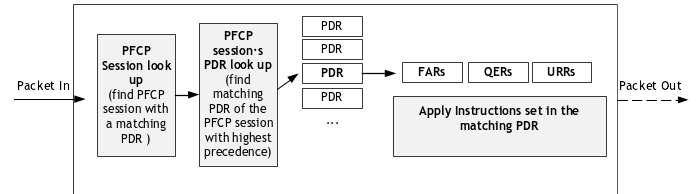
\includegraphics[height=!,width=1\linewidth,keepaspectratio=true]
                    {figures/29_244_5-2-1-1_pack_proc_flow}
    % [] 放的是顯示在 list of figure 的文字
    % {} 放的是顯示在圖下方的文字
    \caption[UP 封包處理流程]{{\footnotesize UP 封包處理流程 (取自 TS 29.244 Figure 5.2.1-1~\cite{3gpp.29.244})}}
    \label{fig:up_pack_proc_flow}
\end{figure}
\pnote{圖片自畫}

圖~\ref{fig:up_pack_proc_flow} 顯示出了 UPF 對於封包的處理過程,當用戶端封包進入後,UPF 會從 PFCP 連線中查找出符合封包的 PDR (PDR 是 UPF 內唯一的),當查找到符合條件的 PDR 後會從 PDR 內儲存的指定 FAR/QER/URR ID 查找相對應的 FAR/QER/URR,來決定針對這個封包相對應的轉送/服務品質/流量計算回報規則,又如果是 FAR 且規則是將封包存入緩衝區,則 FAR 內部可能儲存指定 BAR ID 以查找 BAR 並以此規則對緩衝作出處理方法。

另外在核心網路內部的用戶端則是延用 4G 時期的 GTP (GPRS Tunnelling Protocol) 協定來作為封包的穿隧協議,除了 N6 界面 (UPF 與 DN 的中間界面) 外,核網內的用戶端界面包含 N3 (RAN 與 UPF) 與 N9 (UPF 與 UPF) 都是使用 GTP 協定相連。GTP 協定在封裝時會於網路層 (network layer, l3) 之下再包覆一層 GTP 標頭與新的 IP 標頭,而在有 GTP 標頭的狀況下,UPF 會透過查詢 GTP 內的 TEID 取代查詢傳統 IP 作為識別並作出相對應的轉送動作。而整個用戶端封包流程從手機到網際網路會是,封包從 UE 到 RAN 後會被 RAN 封裝成 GTP 封包並打上核網分配的 TEID,之後封包被送到 UPF,UPF 查看 TEID 透過 PDR 與 FAR 的規則查找,把 GTP 解封裝後送到 DN,完整協定疊 (protocol stack) 如圖~\ref{fig:up_proto}。

\begin{figure}[htbp]
    \centering
    \begin{tikzpicture}
        \tikzset{box/.style={minimum height=2em,draw=black,inner sep=0,thick,node distance=2em},minimum width=5em}
        \def\nflen{2cm}
        % UE
        \node (ue) {UE};
        \node[draw,box,above of=ue] (ue-l1) {L1};
        \node[draw,box,above of=ue-l1] (ue-l2) {L2};
        \node[draw,box,above of=ue-l2] (ue-ip) {IP};
        \node[draw,box,above of=ue-ip] (ue-payload) {Payload};
        % RAN
        \node[right=\nflen of ue] (ran) {RAN};
        \node[draw,box,above of=ran] (ran-l1) {L1};
        \node[draw,box,above of=ran-l1] (ran-l2) {L2};
        \node[draw,box,above of=ran-l2] (ran-under-ip) {{\small under} IP};
        \node[draw,box,above of=ran-under-ip] (ran-udp) {UDP};
        \node[draw,box,above of=ran-udp] (ran-gtpu) {GTP-U};
        \node[draw,box,above of=ran-gtpu] (ran-upper-ip) {{\small upper} IP};
        \node[draw,box,above of=ran-upper-ip] (ran-payload) {Payload};
        % UPF
        \node[right=\nflen of ran] (upf) {UPF};
        \node[draw,box,above of=upf] (upf-l1) {L1};
        \node[draw,box,above of=upf-l1] (upf-l2) {L2};
        \node[draw,box,above of=upf-l2] (upf-under-ip) {{\small under} IP};
        \node[draw,box,above of=upf-under-ip] (upf-udp) {UDP};
        \node[draw,box,above of=upf-udp] (upf-gtpu) {GTP-U};
        \node[draw,box,above of=upf-gtpu] (upf-upper-ip) {{\small upper} IP};
        \node[draw,box,above of=upf-upper-ip] (upf-payload) {Payload};
        % DN
        \node[right=\nflen of upf] (dn) {DN};
        \node[draw,box,above of=dn] (dn-l1) {L1};
        \node[draw,box,above of=dn-l1] (dn-l2) {L2};
        \node[draw,box,above of=dn-l2] (dn-ip) {IP};
        \node[draw,box,above of=dn-ip] (dn-payload) {Payload};
        % line
        % NR
        \draw (ue-l1) -- (ran-l1);
        \draw (ue-l2) -- (ran-l2);
        \draw (ue-ip.east) -- (ran-upper-ip.west);
        \draw (ue-payload.east) -- (ran-payload.west);
        % N3
        \draw (ran-l1) -- (upf-l1);
        \draw (ran-l2) -- (upf-l2);
        \draw (ran-under-ip) -- (upf-under-ip);
        \draw (ran-udp) -- (upf-udp);
        \draw (ran-gtpu) -- (upf-gtpu);
        \draw (ran-upper-ip) -- (upf-upper-ip);
        \draw (ran-payload) -- (upf-payload);
        % N6
        \draw (upf-l1) -- (dn-l1);
        \draw (upf-l2) -- (dn-l2);
        \draw (upf-upper-ip.east) -- (dn-ip.west);
        \draw (upf-payload.east) -- (dn-payload.west);
    \end{tikzpicture}
    % [] 放的是顯示在 list of figure 的文字
    % {} 放的是顯示在圖下方的文字
    \caption[用戶端協定疊]{{\footnotesize 用戶端協定疊}}
    \label{fig:up_proto}
\end{figure}

\subsection{5G 常見流程}
\label{subsec:5g_procedure}

在核心網路中有定義了大量不同的流程~\cite{3gpp.23.502}來適應不同的情境,而其中我們認為有主要四個流程是在核心網路中最重要也是最長觸發的,對這四個流程的觀察可以讓我們對核心網路可以有更快速的瞭解,同時因為其重要性,也適合作為實驗評估時的基準。

\begin{itemize}
\item \textbf{Registration:}
    Registration 是 UE 開啟後第一個所進行的流程,UE 需要透過註冊流程才能跟核心網路索取認證 (authorized)、服務 (services)、移動追蹤 (mobility tracking)、與可達性 (reachability) 等功能。
    並且註冊並不僅僅限於用戶設備連接至核心網路的那一刻,在用戶與核心網路的連接期間,依舊會根據不同的場景執行 Registration,主要分為 Initial Registration,在UE開啟電源後嘗試連接至核心網路時所使用;Periodic Registration,當 UE 處於 CM-IDLE 的狀態時,定期與核心網路回報自身存在;Mobility Registration,當 UE 離開 Registration Area 後到達新的 Tracking Area 後,更新UE狀態時所使用;Emergency Registration,當 UE 僅試圖使用核網所提供的緊急服務時所使用。
    由此可知,只要 UE 試圖與核心網路連結,必定會執行該流程,可見 Registration 在核心網路中的重要性。

\item \textbf{Session Management:}
    5G 核心網路所提供給 UE 的其中一個重要服務即是與資料網路 (Data Network) 的連接,資料網路並不僅限於網際網路 (Internet) 也包含了 IP 多媒體子系統 (IMS) 亦或是私有網路。UE 為了連線至資料網路,將會發起 PDU Session 的建立請求,流程完成後,會建立起UE和資料網路之間的用戶平面,才能進行資料交換。同時在 UE 進行移動時,也可能因為更換 RAN 或甚至 UPF 而需要經常性的作連線的修改 (session modification)。
    如果沒有進行這個流程,UE 將無法連線至網路以獲取所需的資源。

\item \textbf{Handover:}
    換手 (Handover) 為核心網路支援使用者移動性質的關鍵,同時確保服務的連續性。UE 在行動網路供應商提供之服務範圍中移動時,由於從正在提供服務的基地台 (base station, RAN) 所接受訊號變差,UE 為了避免服務品質低落,必須從原先提供服務之基地台切換至其他訊號較強之基地台從而維持相同服務品質,同時必須讓使用者不因切換時所造成的中斷延遲時間而感受到使用體驗上的低落。
    因此換手時間將直接影響了使用者體驗,並且隨著 UE 於長距離下的高速移動,將會大量觸發換手機制,此情形下,確保換手時的低延遲將顯得更為重要。

\item \textbf{Paging:}
    Paging 為核心網路用來尋找 IDLE 狀態中的 UE 並且觸發訊號連接的過程,由於移動設備需要考慮電源管理 (power management),在不需要使用到服務時移動設備會進入 IDEL 狀態來關閉連線以減少電源消耗。
    而在 UE 進入 IDLE 狀態後,若資料網路需要傳送給 UE 的下行封包抵達核心網路,就需要透過 Paging 尋找 UE 接著觸發 Service Request 建立下行 PDU Session,在下行 PDU Session 建立前,所有的下行封包皆由 UPF 進行暫存,等到建立完成後一併轉發。
    因此低延遲的 paging 流程表示能夠讓 UE 即時的接收到下行封包,也降低了 UPF 儲存大量下行封包下的負擔。同時若沒有 paging 流程,UE 將會需要時時保持與核心網路的連線而可能導致大量的電源消耗。
\end{itemize}

\section{現存 5G 核心網路專案}
\label{sec:5g_core_project}

網路上有一些現存的核心網路專案,有一些是開源的有一些則否,像是 NextEPC~\cite{nextepc}、Open5GS~\cite{open5gs}、OpenAir-CN~\cite{oai-cn} 等等,但現行的核心網路專案較少看到符合 3GPP Release 15 (R15)~\cite{3gpp.r15} 的專案,而 free5GC 是其中少數符合 3GPP R15 定義的 5G 核心網路開源專案,透過符合 R15 的核網,我們才能完整測試 3GPP 定義的 5G 功能、接入 5G RAN 作測試與驗證,不需要自己重新完整復刻一個核心網路,而唯有使用開源專案,我們才能快速的開發與修改我們所需要的功能、驗證我們的想法。下面我們介紹一些現存較知名的核心網路專案:

% This LaTeX table template is generated by emacs 27.2
\begin{xltabular}{\textwidth}{|c|c|c|X|}
    \hline
    \textbf{專案} & \textbf{4G/5G} & \textbf{開源} & \multicolumn{1}{c|}{\textbf{描述}} \\
    \hline
    NextEPC~\cite{nextepc} & 4G & v & 網路上以知最完整的 4G 核心網路開源專案,幾乎包含所有 EPC 之功能如 MME、S/P-GW、HSS、PCRF 等,但無 5G 功能。此組織後來開發了 Open5GS 來實作 5G 核心網路。 \\
    \hline
    \shortstack{Open Air\\Interface~\cite{oai}} & 4G & v & OpenAirInterface (OAI) 是一個專注於 4G RAN 的開源專案,爲了驗證其 RAN 之功能,OAI 實作了 OpenAir CN~\cite{oai-cn} 核心網路,但其核心網路僅有部分功能用以驗證 RAN 端,而無實作核網之大部分主要功能。此組織後來有開發 5G 之 RAN 與驗證用 5G 核心網路 OPENAIR-CN-5G~\cite{oai-5gcn},但根據其網頁~\cite{oai-5gc}描述,其核心網路目前僅開源了 AMF、SMF、與 NRF,並無完整網路功能。 \\
    \hline
    \shortstack{Internship\\-5GCN~\cite{intership-5gcn}} & 5G & v & 實作 5G 控制端基於 RESTful SBI 的網路功能,目前僅有 AMF、NRF、SMF、UDM,並未完整實作所有必要功能。 \\
    \hline
    Open5GS~\cite{open5gs} & 5G & v & 基於 NextEPC 發展出的 5G 核心網路,具備大部分 5G R16 所需之網路功能,目前主力開發於 5G NSA 架構,可向下相容 4G EPC,然對於 5G SA 之功能尚不完整。 \\
    \hline
    \shortstack{Metaswitch\\Fusion Core~\cite{metaswitch}} & 5G & x & Metaswitch 是一個基於雲端服務的高效能高可靠度的 5G 核心網路,其支援包含 4G LTE 與 5G NR 的 RAN 接入,其中它更可以支援可程式化的用戶端服務,然而 metaswitch 目前並不提供開源供開發者使用。 \\
    \hline
    free5GC~\cite{free5gc} & 5G & v & 第一個 5G SA 架構的開源專案,目前有實作大部分 5G R15 網路功能,並且有額外實作 non-3gpp 的功能,然而不支援 NSA 架構,並且在可靠性與效能上目前並不完善。 \\
    \hline
    OpenUPF~\cite{openupf} & 5G & v & 基於 3GPP R16 所開發出來的 UPF,底層使用 DPDK 提高高效能轉發,並且可以部屬於 K8S 上提供可擴展性,然而並無實作控制端,僅有用戶端 UPF 功能。 \\
    \hline
    \shortstack{UPF P4\\PoC~\cite{upf-p4-poc}} & 5G & v & 驗證基於 P4 (Programming Protocol-Independent Packet Processors) 實作出 UPF 的概念,目前尚在 PoC 階段並且僅有實作 UPF 部分。 \\
    \hline
    upg-vpp~\cite{upg-vpp} & 5G & v & 基於 3GPP TS 23.214~\cite{3gpp.23.214} 與 TS 29.244~\cite{3gpp.29.244} 所實作的 GTP-U 閘道器 (gateway),底層使用 Cisco 開發的 Vector Packet Processor (VPP)~\cite{fdio.vpp},僅實作 UPF 之功能。 \\
    \hline
    upf-xdp~\cite{upf-xdp} & 5G & v & 基於 Linux Express Data Path (XDP) 所實作之 UPF 的概念性驗證,目前停留於驗證階段且僅實作 UPF 部分。 \\
    \hline
    % [] 放的是顯示在 list of figure 的文字
    % {} 放的是顯示在圖下方的文字
    \caption[5G 專案介紹]{{\footnotesize 5G 專案介紹~\cite{awesome-5g}}}
    \label{tab:5g_proj_intro}
\end{xltabular}


\section{現行方案的挑戰}
\label{sec:challenge}

% 強調 core network 因為 NFV 化,所以不再依賴硬體而可以部屬於同一 host,是否保持用 RPC 溝通就是可以重新審視的問題

\cnote{這邊直接把工具拿出來描述有點怪,需要找一個不突兀的方法把 dpdk 跟 shared memory 帶出來}

\cnote{或在這裡放 related works}

% 其他類似平臺
% 直接用 dpdk, nff-go

\subsection{Data Plane Development Kit}
\label{subsec:DPDK}

\begin{figure}[htb]
    \centering
    % 圖片的高度與寬度, height 設為 ! 代表由寬度大小等比例縮放
    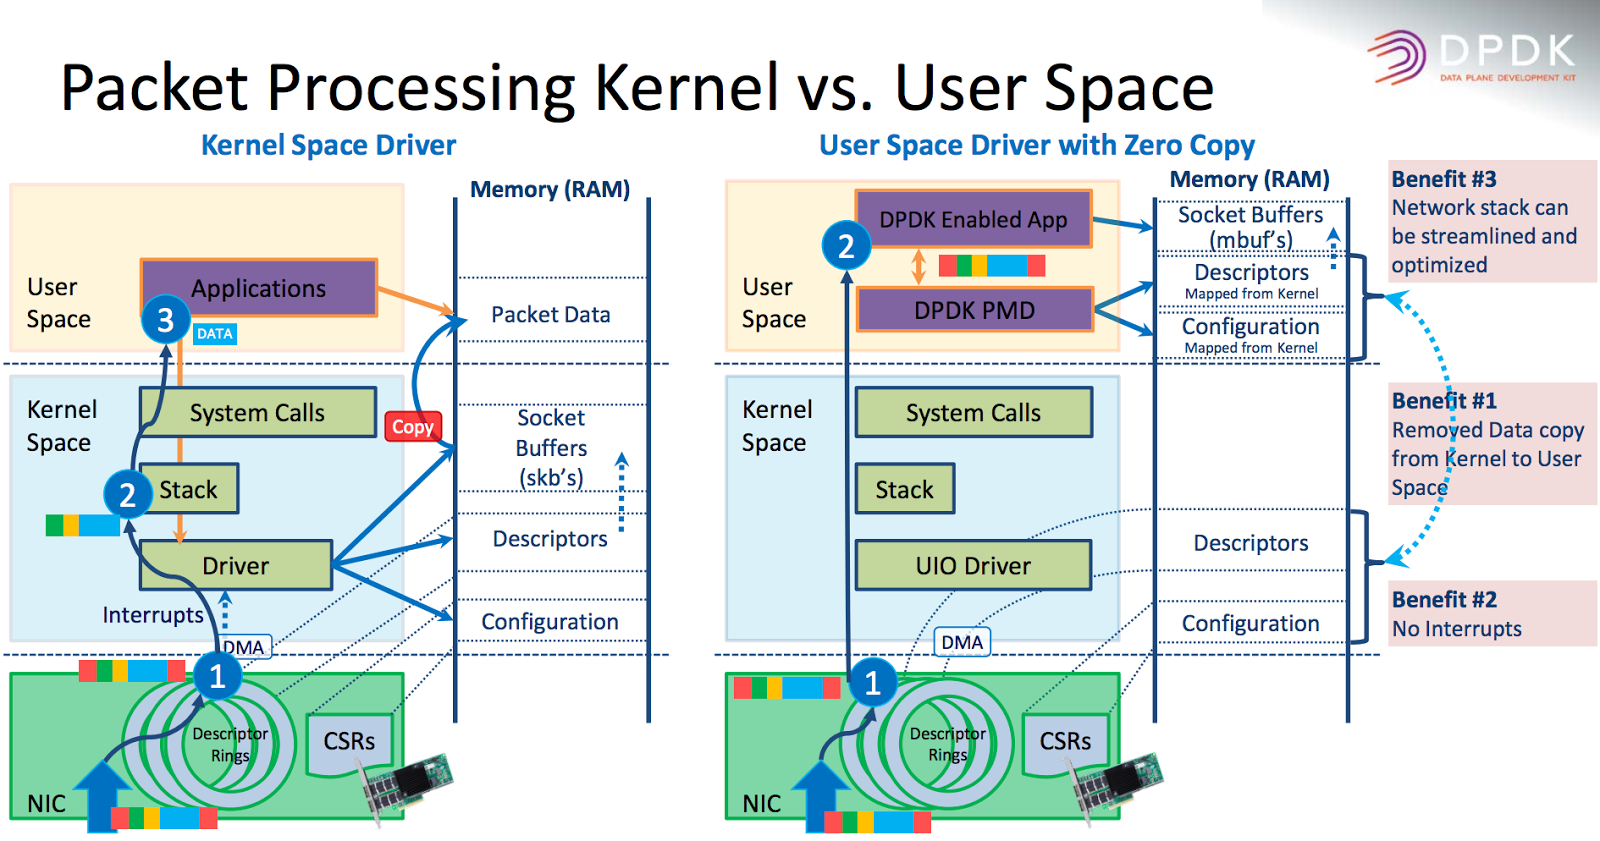
\includegraphics[height=!,width=0.6\linewidth,keepaspectratio=true]
                    {figures/dpdk_vs_kernel}
                    % [] 放的是顯示在 list of figure 的文字
                    % {} 放的是顯示在圖下方的文字
                    \caption[封包處理比較:Linux 核心與 DPDK]{{\footnotesize 封包處理比較:Linux 核心與 DPDK \cite{dpdk}}}
                    \label{fig:dpdk_vs_kernel}
\end{figure}
\pnote{這張圖需要重畫}

\subsection{Shared Memory}
\label{subsec:shared_memory}
